\subsection*{Mört-män}
Baserad på rasen Kua-Toa från \textit{Monster Manual D\&D 5e\cite{MonsterManual}} \\
\url{https://www.dandwiki.com/wiki/Kuo-Toa_(5e_Race)}
%
\subsubsection*{Utseende}
Mört-män är något kortare än människor (medium). De har grå hud, stora gula ögon som skelar och händer samt fötter med simhud och svarta klor. Mört-män är kallblodiga och fuktiga. De uppskattar värme och hög luftfuktighet, varma bad, bastu och eldar.
%
\subsubsection*{Historia}
För hundratals år sedan levde Mört-männen i större samhällen och städer runt Norgerias kuster. Deras magiska och teknologiska egenskaper var på liknande nivå som den moderna människans samhälle, men det är sedan länge bortglömt. Nu lever de i mindre samhällen under ytan.
%
\subsubsection*{Egenskaper}
\textbf{Ability Score Increase.} Your Strength score increases by 2, and your Wisdom score increases by 1. \\
\textbf{Age.} The Kuo-toa age a bit faster than humans, reaching maturity at age 7 and living around half a century. \\
\textbf{Amphibious.} You can breathe in both air and water. \\
\textbf{Darkvision.} You are accustomed to the darkness of the Underdark, where daylight has no power. You can see in dim light within 120 feet of you as if it were bright light, and in darkness 
as if it were dim light. You can't discern color in darkness, only shades of gray. \\
\textbf{Slippery.} You have advantage on Dexterity (Acrobatics) checks and saving throws to escape a grapple or grapple attempt. \\

\begin{figure}
	\centering
	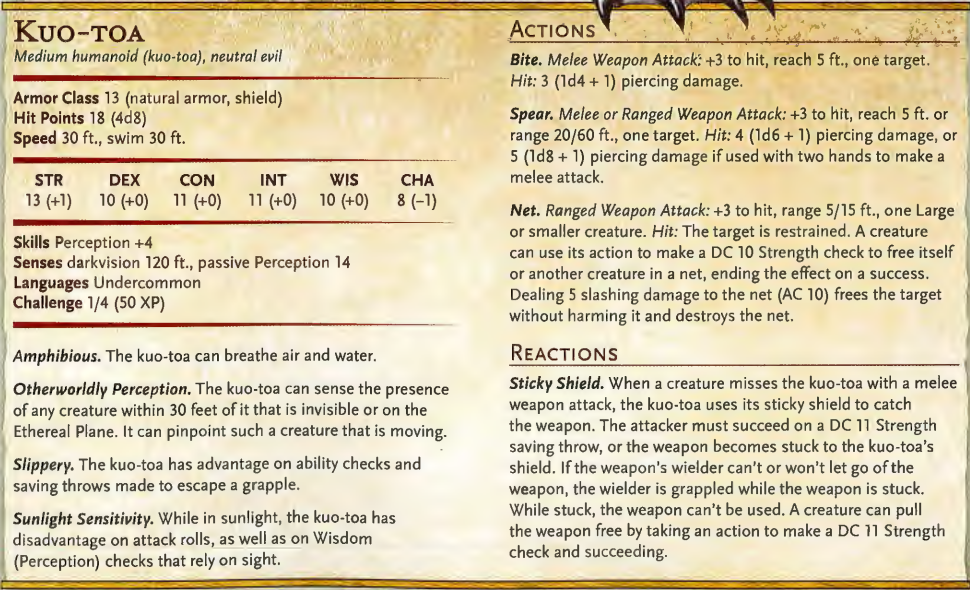
\includegraphics[width=\textwidth]{MortMan}
	\caption{\textit{Kuo-Toa} from \textit{Monster Manual D\&D 5e}\cite{MonsterManual}}
\end{figure}